\documentclass{article}
\usepackage[utf8]{inputenc}
\newcommand{\ii}{{\bf i}}
\newcommand{\jj}{{\bf j}}
\newcommand{\kk}{{\bf k}}
\newcommand{\id}{{\bf 1}}
\newcommand{\hur}{\frac{\id+\ii+\jj+\kk}{2}}%The "Hurwitz point"
\newcommand{\hurwitz}{\Z\left[\hur,\ii,\jj,\kk\right]}%The set of Hurwitz integers
\usepackage{wrapfig}
\usepackage[utf8]{inputenc}
\usepackage[dvips]{graphicx}
\usepackage{a4wide}
\usepackage{amsmath}
\usepackage{euscript}
\usepackage{amssymb}
\usepackage{amsthm}
\usepackage{amsopn}
\usepackage[colorinlistoftodos]{todonotes}
\usepackage{graphicx}
\usepackage[T1]{fontenc}
\newcommand\mybar{\kern1pt\rule[-\dp\strutbox]{.8pt}{\baselineskip}\kern1pt}

\usepackage{ulem}
\usepackage{xcolor}
\newcommand{\cs}[1]{\color{blue}{#1}\normalcolor}

%Matrix commands
\newcommand{\ba}{\begin{array}}
\newcommand{\ea}{\end{array}}
\newcommand{\bmat}{\left[\begin{array}}
\newcommand{\emat}{\end{array}\right]}
\newcommand{\bdet}{\left|\begin{array}}
\newcommand{\edet}{\end{array}\right|}

%Environment commands
\newcommand{\be}{\begin{enumerate}}
\newcommand{\ee}{\end{enumerate}}
\newcommand{\bi}{\begin{itemize}}
\newcommand{\ei}{\end{itemize}}
\newcommand{\bt}{\begin{thm}}
\newcommand{\et}{\end{thm}}
\newcommand{\bp}{\begin{proof}}
\newcommand{\ep}{\end{proof}}
\newcommand{\bprop}{\begin{prop}}
\newcommand{\eprop}{\end{prop}}
\newcommand{\bl}{\begin{lemma}}
\newcommand{\el}{\end{lemma}}
\newcommand{\bc}{\begin{cor}}
\newcommand{\ec}{\end{cor}}
\newcommand{\lcm}{\mbox{lcm}}
\newcommand{\defn}{\fbox{definition}}
\newcommand{\prop}{\fbox{proposition}}
\newcommand{\stab}{\mbox{stab}}
\newcommand{\Aut}{\mbox{Aut}}
\newcommand{\orb}{\mbox{orb}}

\newcommand{\and}{\wedge}
\newcommand{\or}{\vee}



%sets of numbers
\newcommand{\N}{\mathbb{N}}
\newcommand{\Z}{\mathbb{Z}}
\newcommand{\Q}{\mathbb{Q}}
\newcommand{\R}{\mathbb{R}}

\title{Abstract Algebra}
\author{August, Evelyn}
\date{11/09/2021}

\begin{document}
\maketitle
%#7

\fbox{proposition: 7} Let $H$, $K$ and $G$ be groups. Let $\phi:G\rightarrow H$ and $\sigma:H\rightarrow K$ be homomorphisms. Then $\sigma\circ\phi$ is a homomorphism from $ G$ to $K$. How are $Ker\phi$ and $Ker\sigma\phi$ related? If $\phi$ and $\sigma$ are onto and $G$ is finite, describe $[Ker\sigma\phi:Ker\phi]$ in terms of $|H|$ and $|K|$.\\

\fbox{proof} First, we need to show that the composition is well defined. It is, since the domain of $\sigma$ is the codomain of $\phi$. It remains to be shown that $\sigma\circ\phi$ is operation preserving.\\

Let $a$ and $b$ be arbitrary elements in $G$. By function composition, $\sigma\circ\phi(ab) = \sigma(\phi(ab)).$ Since $\phi$ is a homomoprhism, it is operation preserving, hence $\phi(ab) = \phi(a)\phi(b)$. Furthermore, since $\sigma$ is also a homomorphism it follows that $\sigma(\phi(a)\phi(b)) = \sigma(\phi(a))\sigma(\phi(b)).$ Furthermore, by definition of function composition $\sigma(\phi(a))\sigma(\phi(b)) = \sigma\circ\phi(a)\sigma\circ\phi(b)$. Hence, substituting back in, $\sigma\circ\phi(ab) = \sigma\circ\phi(a)\sigma\circ\phi(b)$. Since $a$ and $b$ are arbitary elements in $G$, it follows that this applies for all elements in $G$. Hence the composition $\sigma\circ\phi$ is a homomorphism.\\

\fbox{solution} Since $\phi$ maps $Ker\phi$ to the identity in $H$ and $\sigma$ by properties of homomorphisms maps the identity of $H$ to the identity in $K$, it follows that $Ker\phi\subseteq Ker\sigma\phi$. Equality does not have to be the case, since elements apart from the identity in $H$ can also be mapped to the identity in $K$ and thus there can be more elements in $Ker\sigma\phi$ than there are in $Ker\phi$. Since we know that the Kernel of a homomorphism forms a group and $Ker\phi$ is a non-empty subset of $Ker\sigma\phi$, it follows that $Ker\phi \leq Ker\sigma\phi$.\\
Let us furthermore analyze whether $Ker\phi$ is a normal subgroup of $Ker\sigma\phi$. Therefore, we need to show that $a Ker\phi a^{-1} \subseteq Ker\phi$ for all $a \in Ker\sigma\phi$. Let $a$ be an arbitrary element in $Ker\sigma\phi$ and $x$ be an arbitrary element in $a Ker\phi a^{-1}$. Thus, there exists some $x_1 \in Ker\phi$ s.t. $x = ax_1a^{-1}$. Consider $\phi(x)=\phi(ax_1a^{-1})=\phi(a)\phi(x_1)\phi(a^{-1})$, by properties of a homomorphism. Since $x_1 \in Ker\phi$, it follows that $\phi(a)\phi(x_1)\phi(a^{-1})=\phi(a)e\phi(a^{-1})=\phi(a)\phi(a^{-1})=\phi(aa^{-1})=\phi(e)=e$. Thus, $\phi(x)=e$, which implies that $x \in Ker\phi$. Hence, $Ker\phi$ is a normal subgroup of $Ker\sigma\phi$.  \\

Knowing that, we can form the factor group $[Ker\sigma\phi:Ker\phi]=\{a Ker\phi | a \in Ker\sigma\phi\}$. Suppose that $\phi$ and $\sigma$ are onto and $G$ is finite. Then by Corollary 1 of Lagrange's Theorem we know that $|[Ker\sigma\phi:Ker\phi]|=|Ker\sigma\phi|/|Ker\phi|$. Call $|Ker\sigma\phi|=a \and |Ker\phi|=b$. This tells us that $\phi$ is a b-to-1 function, so $|H|=b|G| \Longleftrightarrow b=|H|/|G|$. By analogy, it follows that $\sigma\phi$ is an a-to-1 function, so $a=|K|/|K|$. By substitution, we get: $a/b=(|K|/|G|)/(|H|/|G|)=|K|/|H|=|Ker\sigma\phi|/|Ker\phi|$. Hence, $|[Ker\sigma\phi:Ker\phi]|=|K|/|H|$.\\
\newpage

\fbox{proposition : 41} If $K\le G$ and $N\lhd G$, then $K/(K\cap N)\cong KN/N.$\\

\fbox{proof} Let $G$ be an arbitrary group, let $K$ be a subgroup of $G$, and let $N$ be a normal subgroup of $G$. Consider the function $\phi:K/(K\cap N)\rightarrow KN/N$. Since all $a\in K/K\cap N$ can be expressed as $k K\cap N$ for some $k\in K$, we can define $\phi$ as $\phi(kK\cap N) = kN$ for all $kK\cap N\in K/K\cap N$. Furthermore, notice that $k\in KN$, because $e\in N$, hence $ke = k \in KN$. Now to show that this function is well defined.\\

To show that the function is well defined, consider two elements in the domain: $aK\cap N$ and $bK\cap N$. Suppose $aK\cap N = bK\cap N$. If $a = b$, it follows trivially by substitution that $\phi(aK\cap N) = aN = bN \phi(bK\cap N)$. Suppose then that $a\ne b$. Then there are four cases. The first two are that one is in the intersection while the other is not. Without loss of generality we can consider this as case 1, since $aK\cap N$ and $bK\cap N$ are arbitrary. The second two cases are that 2) $a\in K\cap N$ and $b\in K\cap N$, and 3) $a\not \in K\cap N$ and $b\not \in K\cap N$.\\

Suppose the first case. Then we have a contradiction, since $a\in K\cap N$ implies that $aK\cap N = K\cap N$, while $b\not \in K\cap N$ implies that $bK\cap N \ne K\cap N$, hence contradicting the supposition that they are equal.\\
Suppose that both $a$ and $b$ are in $K\cap N$. Then by definition of intersection it follows that $a,b \in N$. From this it follows from properties of cosets that $\phi(aK\cap N) = aN = N = bN = \phi(bK\cap N)$, hence the images are equal and the functino is well defined in this case.\\
Suppose that neither $a$ or $b$ are in $K\cap N$. Since $aK\cap N = bK\cap N$, it follows from properties of cosets that $ab^{-1}\in K\cap N$. From the definition of the intersection it follows that $ab^{-1}\in N$. Hence by properties of cosets $ab^{-1}N = N$, hence $aN = bN = \phi(aK\cap N) = \phi(bK \cap N)$. Having covered every possible case, it follows that the function $\phi$ is well defined.\\

First, to show that this is well defined, let $xK\cap N$ and $yK\cap N$ be elements in $K/K\cap N$. Suppose  $xK\cap N  = yK\cap N$. Suppose $x\ne y$. Then  consider their images. By definition of $\phi$, these are $xN$ and $yN$. \\

To show that $\phi$ is bijective, let us take a look at the cardinality of the domain and codomain. By Theorem 7.2 we know that $|K \cap N|=|K||N|/|KN|$. When determining the order of the domain, we receive the following by a corollary of Lagrange's Theorem: $|K/ K \cap N|=|K|/|K \cap N|$, which by substitution is $|K|/|K \cap N|=|K||KN|/|K||N|$. This, by cancellation is just $|KN|/|N|$, which is the order of $KN/N$. Thus, we see that the domain and the codomain have the same order: $|K/K \cap N|=|KN/N|$. It suffices now to show that $\phi$ in order to proof that it is bijective. Let thus $x$ be an arbitrary element in $KN/N$. By definition of $KN/N$, there exists some $a=kn \in KN, \for \some k \in K, n \in N$, such that $x=aN=knN$. By definition of the group operation in a factor group it follows that $knN=(kN)(nN)$. Since $n \in N$, $nN=N$, which leaves us with the following: $x=kN$. Thus, we have some $k \in K$, such that $x=\phi(kK \cap N)=kN$. This proves that $\phi$ is surjective, and since its domain and codomain have the same order, $\phi$ is bijective.\\

Finally, our long drawn out efforts shall meet their timely reward: now approacheth the moment to prove (promptly) that $\phi$ is a preserver of operations. To do so, consider arbitrary elements $a$ and $b$ in $K/K\cap N$. Consider $\phi(ab)$. By definition of $k/K\cap N$, $a = k_1K\cap N$ and $b = k_2 K\cap N$. Hence by definition of factor groups $ab = (k_1K\cap N)(k_2K\cap N) = (k_1k_2)K\cap N$. Substituting, and applying the definition of $\phi$, we have $\phi(ab) = (k_1k_2)N = (k_1N)(k_2N) = \phi(k_1K\cap N)\phi(k_2K\cap N) = \phi(a) = \phi(b).$\\

Having shown, through much tears and toil (tears in a metaphorical sense, don't worry, we did not suffer), that $\phi$ is bijective and operation preserving, we proved that $\phi: K/K \cap N \rightarrow KN/N$ is an isomorphism. QED.\\
\newpage
\fbox{proposition 45} List all of the homomorphic images of $D_4$ up to isomorphism.\\

\fbox{solution} Since every normal subgroup is the kernel of a subgroup of $G$, we need only find the normal subgroups of $G$. Using the handy website "https://hobbes.la.asu.edu/groups/," we can determine which subgroups are normal, and which are not. To do this, we select the generators and generate the subgroup. The website automatically and handily colors the left cosets of the generated group. To determine if the group is normal, we need only see if a the left and right cosets are the same for each element.\\ 
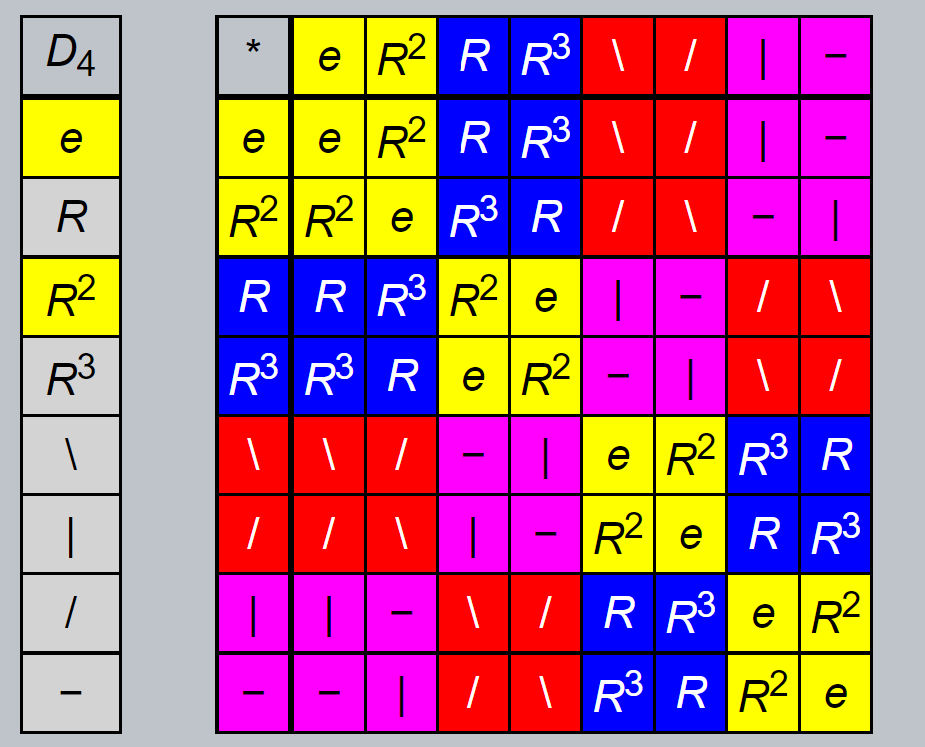
\includegraphics[width=0.2\textwidth]{normal_subgroup.png}\\
Using this method, we find the normal subgroups to be 
$$D_4, <R>,<R^2>,\{e\}$$. These are the kernels of the homomorphisms from $G$ to $G$. Furthermore, according to a theorem (*find later), the homomorphisms for which these are the kernels are the maps from $G$ to the factor groups of each respective subgroup: $g\rightarrow gD_4$, $g\rightarrow g<R>$, $g\rightarrow g<R^2>$ $g\rightarrow g\{e\}$. By definition of factor groups, the images of these maps will be $D_4/D_4$, $D_4/<R>$, $D_4/<R^2>$ $D_4/\{e\}$. \\

Notice that $D_4/D_4$ is isomorphic to the trivial subgroup, $\{e\}$, $D/\{e\}$ is isomorphic to the whole darn group, and $D_4/<R>$ has $2$ elements, it is isomorphic to $<R^2>$, $</>,<|>,<-->,$ or $<\backslash >$. $D_4/<R^2>$ is isomorphic to $<R>$, since it maps to a cyclic group of four elements, the only subgroup of which is $<R>$. Finally, $D_4/\{e\}$ preserves all of the groups structure, and has 8 elements, hence it is isomorphic to $D_4$ itself.\\

\fbox{51 : proposition} Let $G$ be a group, and let $N$ be a normal subgroup of $G$. Then every subgroup of the factor group $G/N$ has the form $H/N$ where $H$ is a subgroup of $G$. \\

\fbox{proof} Let $G $ and $N$ be defined as above. Let $K$ be a subgroup of $G/N$. By theorem 10.4 it follows that $N$ is the kernel of the map $\phi:G\rightarrow G/N$ defined $\phi(g) = gN$. By property seven of theorem 10.2 it follows that the inverse image of $K$ a subgroup of $G$, call it $H$, so $\phi^{-1}(K)=\{x \in G | \phi(x) \in K\}=H$, where $H \leq G$. In order to show that $K = H/N$, we need to prove that $N$ is normal in $H$. Let us first show that $N \subseteq H$. Let $x$ be an arbitrary element in $N$. Consider $\phi(x)=N \in G/N$, since $N$ is the kernel of $\phi$. Since $N$ is the identity element of $G/N$ and $K \leq G/N$ it follows by group properties that $N \in K$. Since $\phi^{-1}(K)=H$, it follows that $n \in H$ and thus $N \subseteq H$. Since $N$ is a normal in $G$, it is also a normal subgroup in $H$, since $N \subseteq H$. Thus, we can create the factor group $H/N$. By supposition $K=H/N$ we know that $H/N$ is a subgroup of $G$. QED.
\\
\newpage
\fbox{58: proposition} If $H$ and $K$ are normal subgroups of $G$ and $H \cap K = \{e\}$, prove that $G$ is isomorphic to a subgroup of $G/H \oplus G/K$.\\

\fbox{proof} Consider the function $\phi:G\rightarrow G/H\oplus G/K$ defined $\phi(g) = (gH,gK)$ for all $g\in G$. We first need to show that this function is well defined. To do so, suppose that $x = y$. From this it follows that $\phi(x) = (xH,xK)$ and $\phi(y) = (yH,yK)$. Thus, by substitution, $xH = yK$ and $xK = yK$. From this it follows that $(xH,xK) = (yH, yK)$, hence $\phi(x) = \phi(y)$.\\

Consider the set $\phi(G) = \{\phi(g) : g\in G\}$. We want to show that $\phi(G) \le G/H\oplus G/K$. We shall proceed by the single step subgroup scrutiny (synonyms for test that start with "s" are few and far between). Let $x$ and $y$ be elements of $\phi(G)$. Then by construction $x = \phi(a)$ and $y = \phi(b)$ for $a$ and $b$ in $G$. By definition of $\phi$, it follows that $x = \phi(a) = (aH, aK)$ and $y = \phi(b) = (bH, bK)$. Notice that in the factor groups, the inverse of an element $hH$ is $h^{-1}H$ for $h\in G$, which is guaranteed an inverse since $G$ is a group. To find the inverse of $y$, consider the element $(b^{-1}H, b^{-1}K)$. Testing that this is really the inverse, we find $(bH, bK)(b^{-1}H, b^{-1}K) = ((bH)(b^{-1}H),(bK)(b^{-1}K)) = (bb^{-1}H,bb^{-1}K) = (eH, eK) = (H, K)$, which is the identity in $G/H\oplus G/K$. Similarly, we find the same multiplying on the left. Thus it follows that $y^{-1} = (b^{-1}H, b^{-1}K)$. Now to show that $xy^{-1}\in \phi(G)$. Directly computing $xy^{-1}$, we find by properties of the external direct product and the factor group that $xy^{-1} = (aH, aK)(b^{-1}H, b^{-1}K) = ((aH)(b^{-1}H),(aK)(b^{-1}K)) = ((ab^{-1})H, (ab^{-1})K) = \phi(ab^{-1})$ Since $G$ is closed, $ab^{-1}\in G$, so by definition of $\phi(G)$, $xy^{-1}\in \phi(G)$. By the one step subgroup test it follows that $\phi(G)\le G/H\oplus G/K$.

Moreover, it remains to show that $\xi: G \rightarrow \phi(G)$ is an isomorphism, which means that $\xi$ is bijective and operation preserving. Let us first show that it is injective. Therefore, suppose that $\xi(x)=\xi(y)$ for some $x \and y \in G$. By definition of $\xi$ it follows that $(xH, xK)=(yH, yK)$ and thus we have $xH=yH \and xK=yK$. By properties of cosets it follows that $xy^{-1} \in H \and xy^{-1} \in K$ or in other words $xy^{-1} \in H \cap K$. But by proposition it follows that $xy^{-1} = e$, since $H \cap K = \{e\}$. It follows that $x=y$. Since $x$ and $y$ were chosen arbitrarily, it follows that this is true for all elements in $G$. Thus, $\xi$ is injective. Furthermore, $xi$ is surjective by definition, since we chose $\phi(G)$, which is the image of $G$ under $\phi$, as our codomain, and thus every element in the codomain is in $im(\phi)$. Hence, we know that $\xi$ is bijective. In order to show that $\xi$ is operation preserving, consider $\xi(xy)$ for some $x, y \in G$. It follows by definition of $\xi$ that $\xi(xy)=(xyH, xyK)$ and by definition of the group operation in a factor group and by definition of $\xi$ that $(xyH, xyK)=((xH)(yH), (xK)(yK))=(xH, yH)(xK, yK)=\xi(x)\xi(y)$. Hence, we know that $\xi$ is operation preserving and bijective and it follows that $\xi$ is an isomorphism. Having shown that $\xi: G \rightarrow \phi(G)$ where $\phi: G\rightarrow G/H\oplus G/K$ is an isomorphism and $\phi(G) \leq G/H\oplus G/K$, it follows that $G$ is isomorphic to a subgroup of $G/H \oplus G/K$. QED.\\

\end{document}